\NeedsTeXFormat{LaTeX2e}

\documentclass[12pt]{article}

\usepackage{amsmath}

% The above lines establish the type of LaTeX you're using, the font and the general
% type of document (article, book, letter).


% Various bold symbols - optional stuff
\providecommand\bnabla{\boldsymbol{\nabla}}
\providecommand\bcdot{\boldsymbol{\cdot}}
\newcommand\etb{\boldsymbol{\eta}}

% For multiletter symbols - optional stuff
\newcommand\Imag{\mbox{Im}} % cf plain TeX's \Im
\newcommand\Ai{\mbox{Ai}}            % Airy function
\newcommand\Bi{\mbox{Bi}}            % Airy function


% array strut to make delimiters come out right size both ends
\newsavebox{\astrutbox}
\sbox{\astrutbox}{\rule[-5pt]{0pt}{20pt}}
\newcommand{\astrut}{\usebox{\astrutbox}}

% optional shortcuts defined with \newcommand command
\newcommand\p{\ensuremath{\partial}}
\newcommand\tti{\ensuremath{\rightarrow\infty}}
\newcommand\kgd{\ensuremath{k\gamma d}}
\newcommand\shalf{\ensuremath{{\scriptstyle\frac{1}{2}}}}
\newcommand\sh{\ensuremath{^{\shalf}}}
\newcommand\smh{\ensuremath{^{-\shalf}}}
\newcommand\squart{\ensuremath{{\textstyle\frac{1}{4}}}}
\newcommand\thalf{\ensuremath{{\textstyle\frac{1}{2}}}}
\newcommand\ttz{\ensuremath{\rightarrow 0}}
\newcommand\ndq{\ensuremath{\frac{\mbox{$\partial$}}{\mbox{$\partial$} n_q}}}
\newcommand\sumjm{\ensuremath{\sum_{j=1}^{M}}}
\newcommand\pvi{\ensuremath{\int_0^{\infty}%
  \mskip \ifCUPmtlplainloaded -30mu\else -33mu\fi -\quad}}

\newcommand\etal{\mbox{\textit{et al.}}}
\newcommand\etc{etc.\ }
\newcommand\eg{e.g.\ }


%%%%%%%%%%%%%%%%%%%%%%%%%%%%%%%%%%%%%%%%%%%%%%%%%%%%%%%%%%%%%%

% FOR PDFLATEX:  YOU MAY NEED TO (UN)COMMENT THE FIRST LINE DEPENDING ON YOUR (PDF)LATEX DISTRO
%\newif\ifpdf\ifx\pdfoutput\undefined\pdffalse\else\pdfoutput=1\pdftrue\fi
\newcommand{\pdfgraphics}{\ifpdf\DeclareGraphicsExtensions{.pdf,.jpg}\else\fi}

\usepackage{graphicx} % Include figure files
%\usepackage{epsfig}  % old
\usepackage{bm}% bold math

\usepackage{amsfonts}
\newcommand{\field}[1]{\mathbb{#1}}
\newcommand{\C}{\field{C}}
\newcommand{\R}{\field{R}}

\def\eg{{e.g.\ }}
\def\etc{{etc.\ }}
\def\etal{\mbox{\it et al.\ }}

%%%%%%%%%%%%%%%%%%%%%%%%%%%%%%%%%%%%%%%%%%%%%%%%%%%%%%%%%%%%%%%
%%%%%%%%%%%%%%%%%%%%%%%%%%%%%%%%%%%%%%%%%%%%%%%%%%%%%%%%%%%%%%%

% \linespread{2}  UNCOMMENT this for Double Spacing; I think it looks awful.  Most values work, i.e.. 1.67

% it all starts here

\begin{document}

% \pdfgraphics

\section*{Final Project - Planetary Collision}  % No Section number because I used \section* not \section
                                                                           % same thing works for \equation*

\medskip
\noindent % I tend to begin a document with no indentation ... you decide.
Sai Chikine \& Alex Rybchuk

\section{Project Overview}  
Alex Rybchuk$'$s and Sai Chikine$'$s project is the modeling of the collision of two Jovian planets, which was inspired by Chapter 4 of \textbf{Numerical Methods in Astrophysics}. The modeling of the collision of these planets will be accomplished through an approach known as SPH (Smoothed Particle Hydrodynamics). Astrophysical simulations are broadly separated into 2 types of simulations: mesh based and particle based code. 
\newline \indent
SPH is a particle based system, which approximates a fluid medium as a collection of a large number of particles, each possessing the fluid properties that the simulation aims to track and model. Each particle is treated as a point when subjected to forces and interactions, but, it also has a 'cloud' of other properties that cannot be applied to single points, such as density or pressure, which depend on volume or area. Essentially, SPH models interactions of point particles, but each of these point particles has 3-D properties. These 3-D properties are evaluated using a \textbf{smoothing kernel}, which is a function that assigns a value based on a distance away from the particle. This function could be anything, and one that is commonly used is a Gaussian. The Gaussian distribution makes sense, since the property in question of the fluid is strong closest to it and drops off as one gets farther away. A parameter called the \textbf{smoothing length} is involved here, which is a way to tune how far away particles can be and still affect each other. SPH based simulations have distinct advantages over mesh based ones, such as the ability to deal with large empty spaces efficiently (since those areas are not contributing to computation time), and the ability to deal with asymmetric models more easily (since symmetries are often needed in mesh based codes to set boundary conditions; SPH codes need no boundary conditions). 
\newline  \indent
In light of these advantages, SPH simulations are often used to model large systems, such as galaxies or universes. They are also often used to simulate systems such as gas giants, stars, and supernovas, since these situations are modeled well with a fluid model and can result in complex asymmetries. This project aims to utilize an SPH simulation to model the collision of two gas giants. These gas giants will be modeled as \textbf{polytropes}, which are gasses whose pressure only depends on density. Since gravity force also depends on density, we have a simple equilibrium condition to be fulfilled between pressure and gravity.
\newline\indent
In the end, we obtain a model given by 4 1st order ODEs. These ODEs would evolve the system through time based on a pressure force and a gravity force, essentially giving us an N-Body simulation with an added pressure force to be taken into account. The aim of the project was to create two collections of gasses that would reach an equilibrium state, and then collide these newly formed planets to see what would happen. There have been many implementations of gas giants or small stars using SPH code, and these examples of previous work were used as references for our project. Many implementations used slightly different approaches than the one our textbook led us down. Nonetheless, the area of astrophysical simulations using SPH code is an active area of current work and research, and it was our hope to train ourselves on this exciting physics tool.

\section{Member Roles}
Alex was responsible for the code involving the smoothing kernel and the gradient of the smoothing kernel, and was largely responsible for the initial prototype off of which our project then evolved. Sai was then largely responsible for the gravity code as well as the 3d implementation of our project. Initially, member roles and contributions were imagined to be quite different than they turned out, but due to a large amount of unforeseen difficulty, both members ended up contributing to most of the code, and a large amount of time was spent tweaking and troubleshooting. Originally, Alex was supposed to be responsible for the core code, and Sai was to be responsible for the enhancements and improvements. However, the core code proved to immensely difficult to get into a functional state, so the roles broke down into what they were in the end. 

\section{Approach}
Our approach to the problem followed the textbook's approach very closely. In SPH, particles are evolved through time according to a \textbf{gravity force}, and a \textbf{pressure force}. These two forced need to be coupled somehow in order for equilibrium to be reached. In our case, they were coupled through the polytropic relation: $P=K\rho^{\gamma}$, where K is a constant which depends on the planet being modeled and gamma depends on the type of polytrope being modeled. In our case, $\gamma$ was 2.
\newline\indent
Pressure and density of the particles were updated with each time step, which allowed the pressure force to change accordingly. The particles were divided into particles of equal mass, which was not updated, so the gravity force was only updated based on distances between particles. Gravity was also truncated at a certain distance, known as the gravity cutoff length, so that gravity forces did not grow to infinite in magnitude as particles got very close together. From here, the problem was essentially treated as an N-Body problem. The N-Body problem was evolved through time simply with $O(N^2)$ complexity for both gravity and pressure, since planned optimizations and speed-ups would have taken too much time to implement. Each particle's force contribution from each other particle due to gravity and pressure was summed, and then the particle's velocity was evolved through time using Euler's Method (RK1). Euler's method was chosen since it was faster than higher complexity methods, and speed was of the essence since we needed to prototype different iterations rapidly. Arrays were created for Velocity, Position, and Density, which contained data for all the particles in our simulation. Each of these arrays were updated during every time step. 
\newline\indent
The initialization of particles was an area in which our project diverged from the textbook approach. The textbook advised us to start with a distribution of particles arranged in annular cells that would preserve the known analytic solution to the system of coupled differential equations which were used to model the system. However, we could not obtain reasonable results with this distribution, since the textbook's description of how to arrange the particles was in a normalized coordinate system, and our simulation was not in a normalized coordinate system. We decided to use a truncated radial Gaussian distribution instead to distribute the particles around a given centerpoint.
\newline\indent
The particles' masses were chosen to recover the total mass of Jupiter, while their densities were initialized according to the smoothing function. A velocity proportionate damping force was also artificially added to model the damping of energy in fluids due to factors such as shocks and thermal dissipation. From here, fine tuning of parameters was needed to reach an equilibrium point. The parameters varied included $K$ (the polytropic constant), $h$ (the smoothing length), the gravity cutoff length, the size of the time step, and the damping constant. Some combinations resulted in our planet blowing apart, while others results in a singularity. However, we were able to reach a stable configuration where the planet converged to a stable size and was in equilibrium.
\newline\indent
The problem was solved in both 2D and 3D separately, since it was believed that these 2 approaches might result in different results since 3D and 2D models possess different symmetries.
\newline\indent
In both 2D and 3D, an equilibrium solution was evolved in time until it had reached equilibrium. To save computation time for the collision, the results from this simulation were saved into a file which served as a starting point for the collision part of our project. Two previously equilibriated planets were initialized and sent racing towards each other to collide.

\section{Ph 235 Topics}

The fundamentals to SPH code include the the basic time evolution of particles based on pressure gradients and gravitational gradients. To handle the problem of discretely computed gradients at single points, points are broken up into smoothing kernels that split a single massive particle into a distribution of mass density. Pressure and density are related using a polytropic equation of state, and the gravitational and pressure contributions to each packet of mass can be evolved in time. An Euler approach was chosen over higher complexity methods to save time. 
\newline\indent
There are Improvements to the code make the code more accurate and more computationally efficient, many of which were explored in class. Some of these improvements include: more accurate initial conditions, a better smoothing kernel approach, involving a tree method into computing forces, and using a variable smoothing length. Careful consideration of initial conditions yield more realistic results, since a random distribution could lead to large local pressure gradients, which is not physically realistic. In addition, more accurate initial conditions would lead to less computational time spent on reaching equilibrium, since the planet would start closer to equilibrium. An improvement on the smoothing kernel would only include force contributions on scales that make sense, instead of summing over all particles in the system, which is computationally inefficient. 
\newline\indent
A tree method of computing, such as the Barnes Hut tree method, was considered to handle the N-Body aspect of our problem. This tree method basically treats groups of particles far away from the particle of interest as a single particle, with the size of the groups increasing as the distance from the particle of interest increases. This leads to a much faster calculation time than the brute force approach we researched. Other methods, such as FMM (Fast Multipole Method), were also researched, but was discounted on account of its programming complexity. Although much time was spent researching the tree method, it was eventually shelved to make time to work on getting the more fundamental parts of the code to work properly. 
\newline\indent
Future improvements to code would definitely include a more efficient N-Body algorithm, such as a tree method or FMM. Finally, introducing a variable smoothing length leads to increased computational efficiency by increasing the length scale of force computations for particles that are more isolated than others.


\section{Evaluation and Discussion}
We were able to achieve a stable equilibrium of an initial Gaussian distribution of particles. These particles converged to a stable size and stopped moving for the most part. The 2D model seemed to collapse uniformly and halt at a certain radius, while the 3D model collapsed quite far, and then pushed back out into an equilibrium size. This deviation in behavior of the 2 models is strange, and further research and investigation is required to understand why it happens. Although the equilibrium behavior was stable, the collision simulation did not yield sensical results. The 2D simulation did not work at all, while the 3D collision simulation yielded results that diverged wildly from the previous examples and literature that was used for reference. It is currently unknown why this happened. However, part of it could have to do with our initial distribution of masses, which diverged from the textbook's approach. Furthermore, our damping scale may have been off (either too much or too little) in the collision part of the code, resulting in an equilibrium solution but not physically realistic results for a collision, where more complex things are happening. Further work could be done in improving the code to make it more physically accurate.
\newline\indent
The final project we ended up with was not quite what we had envisioned when we set out to model a gas giant collision. We ended up with a much more rudimentary product than we had hoped for. The reason for this was in large part due to a lack of understanding of the true difficulty of the problem we had decided to tackle; the literature and references we were using were written by masters students or were masters theses. Another big factor was our unfamiliarity with SPH code in general. A lot of time was spent figuring out how SPH worked, and how the general flow of the problem should look like. Difficulties were also encountered in computing power available, since each iteration took a while to run, and so tuning our parameters took quite a while to reach sensible results. Easy parts of the project were in setting up the overarching structure of the code, including setting up the Euler's method loop, the visualization, and the general coding aspects of the code, such as working with numpy arrays. 
\bigskip

\section{Appendix}


\begin{figure}
\begin{align}
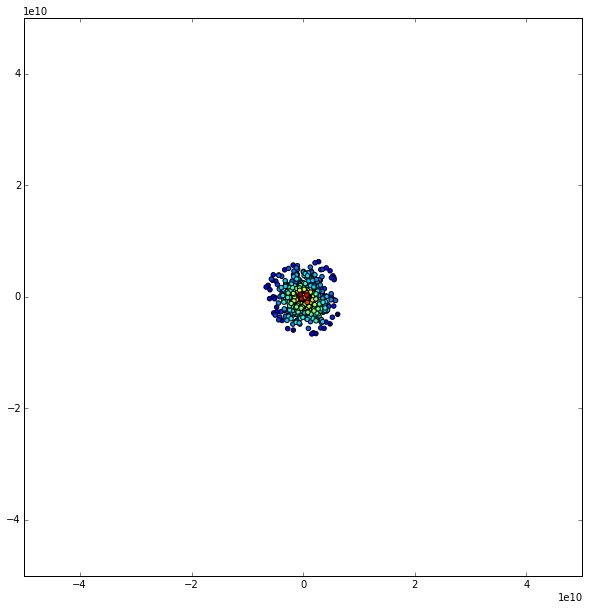
\includegraphics[width=4.0in]{2d_eqb_before.png}
\end{align}
\caption{A randomized initial state of particles in 2D}
\end{figure}

\begin{figure}
\begin{align}
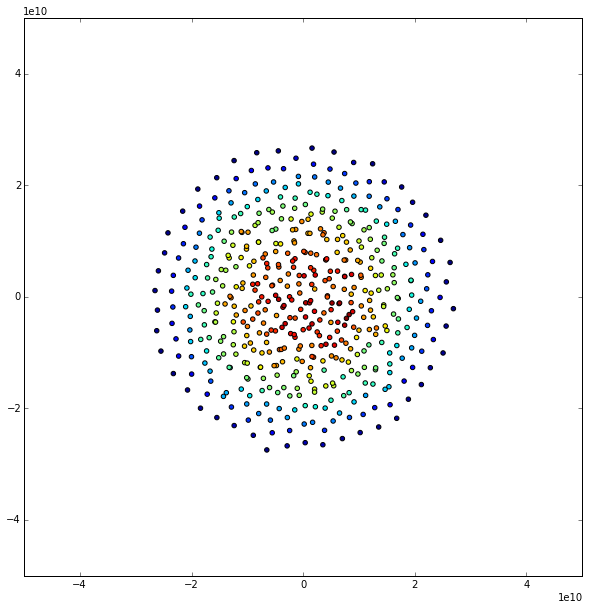
\includegraphics[width=4.0in]{2d_eqb_after.png}
\end{align}
\caption{After 500 times steps, the 2D particles reach equilibrium}
\end{figure}

\begin{figure}
\begin{align}
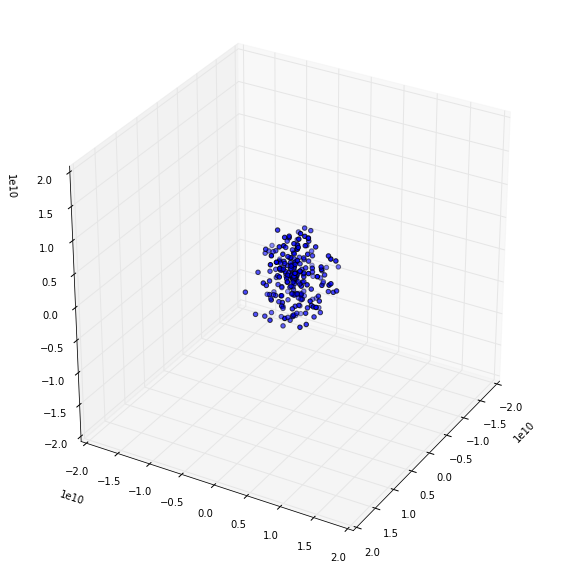
\includegraphics[width=4.0in]{3d_eqb_before.png}
\end{align}
\caption{A randomized initial state of particles in 3D}
\end{figure}

\begin{figure}
\begin{align}
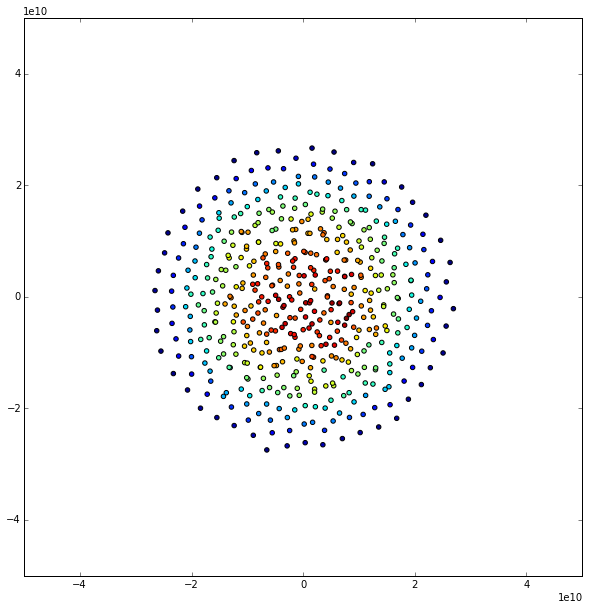
\includegraphics[width=4.0in]{2d_eqb_after.png}
\end{align}
\caption{After 500 times steps, the 3D particles reach equilibrium}
\end{figure}

\begin{figure}
\begin{align}
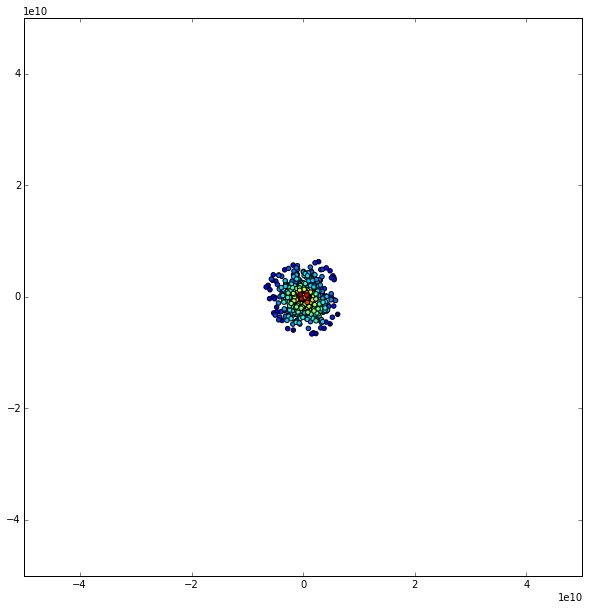
\includegraphics[width=4.0in]{2d_eqb_before.png}
\end{align}
\caption{A randomized initial state of particles in 2D}
\end{figure}



\end{document}